\chapter[Fundamentação Teórica]{Fundamentação Teórica}

Nesta seção são abordados conceitos fundamentais para a compreensão deste trabalho, assim como tendências atuais da literatura em relação ao tema estudado.

\section{Regressão Linear}

Os modelos de regressão linear constituem uma classe de modelos que utilizam funções lineares com parâmetros ajustáveis. O exemplo mais simples dessa classe é a função que realiza a combinação linear das entradas com os parâmetros ajustados para gerar uma predição (eq. \ref{eq:lin_expandida}).

\begin{equation}
    \hat{y} = w_0 + w_1x_1+ ... + w_px_p = \sum_{i = 0}^{p} w_iX = XW
    \label{eq:lin_expandida}
\end{equation}

Onde, $X$ e $W$ correspondem, respectivamente, ao vetor de entradas e de parâmetros, $p$ corresponde ao número de dimensões da variável de entrada e $x_0 = 1$.

Modelos mais complexos e de maior aplicabilidade podem ser obtidos ao se considerar um conjunto fixo de 
transformações não-lineares ($\phi_n(X)$) em vez das variáveis originais, ou em conjunto com elas. 
Esses modelos são lineares em relação às suas variáveis independentes, porém são não-lineares em relação às variáveis de entrada \cite{bishop_2006}.

\subsection{Treinamento de modelos lineares}

O treinamento de modelos lineares consiste em encontrar o vetor de parâmetros $W$ que maximize a similaridade entre o modelo e o sistema modelado. Esse treinamento é normalmente realizado minimizando-se o somatório dos erros quadráticos (eq. \ref{eq:sq_error}) em função do vetor $W$.

% \begin{align}
% \begin{split}
%       E_{sq}(W) {}&= \frac{1}{2} \sum_{n = 1}^{N}\left(y_n-\hat{y}_n\right)^2 = \frac{1}{2} \sum_{n = 1}^{N} \left(y_n-\phi(X_n)W\right)^2
%     \label{eq:sq_error}  
% \end{split}\\
% \begin{split}
%     \pdv{E_{sq}(W)}{W} {}&= \sum_{n = 1}^{N} \phi(X_n)^T\left(\phi(X_n)W - y_n\right)
%     \label{eq:min_sq_error}
% \end{split}
% \end{align}

\begin{equation}
\begin{split}
      E_{sq}(W) {}&= \frac{1}{2} \sum_{n = 1}^{N}\left(y_n-\hat{y}_n\right)^2 \\
      &= \frac{1}{2} (Y-\hat{Y})^T(Y-\hat{Y})\\
      &= \frac{1}{2} \left( Y^TY - 2 \hat{Y}^TY + \hat{Y}^T\hat{Y} \right)\\
      &= \frac{1}{2} \left( Y^TY - 2 W^TX^TY + \sum_{n = 1}^{N}\left(X_nW \right)^2 \right)
    \label{eq:sq_error}  
\end{split}
\end{equation}

\begin{equation}\begin{split}
    \pdv{E_{sq}(W)}{W} &= \frac{1}{2} \left( 0 - 2 X^TY + 2\sum_{n = 1}^{N}\left(X_n^TX_n \right)W  \right) \\
    &= - X^TY + X^TX W
    \label{eq:min_sq_error}
\end{split}\end{equation}

Igualando-se a eq. \ref{eq:min_sq_error} a zero e isolando o vetor $W$, obtém-se a eq. \ref{eq:lsnormal}, conhecida como a equação normal para o problema dos mínimos quadrados.

\begin{equation}\begin{split}
    X^TX W &= X^TY \\
    W &= (X^TX)^{-1}X^TY \\
    W &=X^+ Y
    \label{eq:lsnormal}
\end{split}\end{equation}

O termo $(X^TX)$ pode se aproximar de uma matriz singular se muitas das variáveis envolvidas forem linearmente dependentes, resultando assim em dificuldades para o cálculo numérico dos valores e possivelmente em um vetor de parâmetros de alta magnitude. Um termo de regularização pode ser adicionado na eq. \ref{eq:sq_error} 
para minimizar esse problema, garantindo que a nova matriz não é singular.

A adição do termo de regularização tem ainda o efeito de limitar a complexidade efetiva do modelo, reduzindo o \textit{overfitting} e possibilitando a utilização de conjuntos de dados menores \cite{bishop_2006}.

Comumente utiliza-se a norma-L2 do vetor de parâmetros como termo de regularização, dando origem a \textit{ridge regression}. A dedução da equação normal com termo de regularização é análoga à apresentada e resulta na eq. \ref{eq:lsnormal_reg}.

\begin{equation}\begin{split}
    W &= (\lambda I + X^TX)^{-1}X^TY = A^{-1}X^TY
    \label{eq:lsnormal_reg}
\end{split}\end{equation}


\section{Validação Cruzada}

A validação cruzada (\textit{cross-validation}) é um conjunto de metodologias de treinamento e validação que, de maneira simples e efetiva, permitem a estimativa do erro de generalização do modelo.

No método \textit{k-fold} de validação cruzada, os dados de treinamento são divididos em \textit{k} conjuntos aleatórios de tamanhos aproximadamente iguais. Realizada essa divisão, a cada iteração do treinamento, os parâmetros do modelo são determinados utilizando \textit{k}-1 conjuntos e sua performance é avaliada no conjunto restante. O processo se repete até que todos os \textit{k} conjuntos tenham sido utilizados para avaliação e a média das performances observadas fornecem uma estimativa da performance de generalização do modelo \cite{overfitting_crossval}. O algoritmo é ilustrado na Figura \ref{fig:k-fold-cross}.

\begin{figure}[H]
    \centering
    \caption{Validação cruzada: \textit{5-fold}.}
    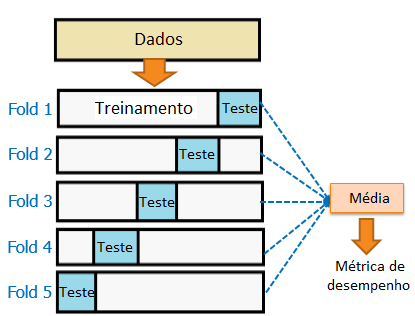
\includegraphics[width=0.7\textwidth]{imgs/rev/cross_validation}
    \legend{\textit{Fonte: Different types of Validations in Machine Learning (Cross Validation)} \cite{cross_val}}
    \label{fig:k-fold-cross}
\end{figure}

Um caso especial do método de validação descrito é o \textit{leave-one-out cross-validation} (LOOCV), onde k é igual ao total de amostras disponíveis (N), ou seja, o treinamento é realizado N vezes com N-1 amostras, e validado na amostra excluída. Tal abordagem apesar de apresentar, em geral, um custo computacional elevado, resulta em um modelo com menor variabilidade e viés para modelos de regressão linear \cite{burman}, produzindo assim resultados com melhor performance e menos \textit{overfitting}.

\subsection{ \textit{Leave-one-out Cross-validation} e Regressão Linear}

Especificamente para o caso do preditor linear, é possível determinar o resultado do LOOCV sem a necessidade de se calcular N preditores, tornando essa uma estratégia interessante para determinar a capacidade de generalização de um modelo linear. A seguir uma dedução adaptada de \cite[p. 268]{lin_reg_analysis} é apresentada.

O erro de LOOCV corresponde à média dos erros quadráticos de cada estimador obtido excluindo-se uma amostra. 

\begin{equation}
    LOOCV = \dfrac{1}{N} \sum_{i=1}^{N}e^2_{[i]}
    \label{eq:cv_error}
\end{equation}
\begin{equation}
    e_{[i]} = y_i - \hat{y}_{[i]} = y_i - x_iW_{[i]} 
    \label{eq:ith_error}
\end{equation}
Onde o $i$ indexa a amostra excluída no treinamento, $\hat{y}_{[i]}$ corresponde à saída do preditor calculado sem a
amostra $(x_i,y_i)$ e $W_{[i]}$ os parâmetros desse preditor.

Pode-se definir o vetor de parâmetros $W_{[i]}$ conforme a eq. \ref{eq:wi}.
\begin{equation}
    W_{[i]} = A_{[i]}^{-1}X_{[i]}^TY_{[i]}
    \label{eq:wi}
\end{equation} 

É possível perceber as seguintes igualdades:
\smallskip\noindent
\begin{equation}
    \begin{split}
        A_{[i]} &= \lambda I + X_{[i]}^TX_{[i]} \\
                &= \lambda I + X^TX - x_i^Tx_i \\
                &= A - x_i^Tx_i    
    \end{split}
    \label{eq:ai_identity}
\end{equation} 

\begin{equation}
    X_{[i]}^TY_{[i]} = X^TY - x_i^Ty_i
    \label{eq:X_iY_i_identity}
\end{equation} 

Aplicando a formula de Sherman–Morrison à eq. \ref{eq:ai_identity}, temos:
\smallskip\noindent
\begin{equation}
    \begin{split}        
       h_i &= x_iA^{-1}x_i^T \\
       A_{[i]}^{-1} &= A^{-1} + \dfrac{A^{-1}x_ix_i^TA^{-1}}{1-h_i}
    \end{split}
    \label{eq:sherman}
\end{equation}

Substituindo as eq. \ref{eq:X_iY_i_identity} e \ref{eq:sherman} na eq. \ref{eq:wi}.
\smallskip\noindent
\begin{equation}
    \begin{split}
        W_{[i]} &= \left(A^{-1} + \dfrac{A^{-1}x_i^Tx_iA^{-1}}{1-h_i}\right) \left(X^TY - x_i^Ty_i\right)\\
                &= W - A^{-1}x_i^Ty_i + \dfrac{A^{-1}x_i^Tx_iW}{1-h_i} - \dfrac{A^{-1}x_i^Tx_iA^{-1}x_i^Ty_i}{1-h_i} \\
                &= W - \dfrac{A^{-1}x_i^T}{1-h_i}\left(  y_i(1-h_i)-x_iW  + h_iy_i \right)  \\
                &= W - \dfrac{A^{-1}x_i^T}{1-h_i}\left(  y_i-\hat{y}_i \right)  \\
    \end{split}
    \label{eq:wi_expandido}
\end{equation}

Substituindo a eq. \ref{eq:wi_expandido} na eq. \ref{eq:ith_error}.
\smallskip\noindent
\begin{equation}
    \begin{split}
        e_{[i]} &= y_i - x_iW_{[i]} \\
                &= y_i - x_i\left( W - \dfrac{A^{-1}x_i^T}{1-h_i}\left(  y_i-\hat{y}_i \right) \right) \\
                &= y_i - \hat{y}_i + \dfrac{h_i}{1-h_i}\left(  y_i-\hat{y}_i \right) \\
                &= \dfrac{y_i- \hat{y}_i}{1-h_i}
    \end{split}    
    \label{eq:ith_error_expandido}
\end{equation}

Seja $P$ a matriz de projeção \cite[p. 303]{applied_matrix_algebra} do preditor (também conhecida como matriz chapéu
 \cite[p. 266]{lin_reg_analysis}) e a matriz de aniquilação $M$ \cite[p. 18]{econometrics} definidas conforme a eq. \ref{eq:proj_res_matrix}
\smallskip\noindent
\begin{equation}
    \begin{split}
        \hat{Y} &= PY \implies P = XA^{-1}X^T \\
        MY &= Y - \hat{Y} \implies M = I - P = I - XA^{-1}X^T
    \end{split}    
    \label{eq:proj_res_matrix}
\end{equation}

Para cada índice $i$, o numerador da eq. \ref{eq:ith_error_expandido} corresponde a linha de mesmo índice da matriz $MY$. 
Além disso o denominador da equação corresponde ao elemento da diagonal da matriz $M$ de mesmo índice. 
A partir dessas observações, pode-se agrupar todos os valores de $e_{[i]}$ na forma da matriz $E_{LOOCV}$, conforme a equação \ref{eq:e_cv}.
\smallskip\noindent
\begin{equation}
    \begin{split}
        E_{LOOCV} = diag(M)^{-1}MY
    \end{split}    
    \label{eq:e_cv}
\end{equation}

Assim, a equação \ref{eq:e_cv}, juntamente com o conhecimento que $M$ é uma matriz simétrica \cite{stats_models}, permite reescrever a eq. \ref{eq:cv_error} na forma matricial apresentada na equação \ref{eq:LOOCV_error}.

\begin{equation}
    \begin{split}
        LOOCV   &= \dfrac{1}{N} \sum_{i=1}^{N}e^2_{[i]} \\
                &= \dfrac{1}{N} E_{LOOCV}^2 \\
                &= \dfrac{1}{N}E_{LOOCV}^TE_{LOOCV} \\
                &= \dfrac{1}{N} (MY)^T\ diag(M)^{-2}MY \\
    \end{split}
    \label{eq:LOOCV_error}
\end{equation}

\section{Aprendizado Incremental}

A atualização dos parâmetros do modelo de regressão linear para uma nova amostra pode ser realizada de maneira incremental, sem a necessidade de se calcular um novo modelo \cite{mit_onlinereg}. Neste trabalho, porém, é de interesse calcular a atualização incremental ao se adicionar uma nova variável. Em especial, é de interesse a determinação de uma forma fechada para a matriz de aniquilação, usada no cálculo do erro de validação cruzada.

A matrizes de interesse para o problema de dimensão $p+1$ tem a forma descrita na eq. \ref{eq:inc_matrix} 
\begin{equation}
    \begin{split}
    X_{p+1} &= \left[\mathbf{X_p}\ x_{p+1}\right] \\
    Y_{p+1} &= \left[\mathbf{Y_p}\ y_{p+1}\right] \\
    A_{p+1} &= (X_{p+1}^T X_{p+1} + \lambda I ) = 
    \begin{bmatrix}
        \mathbf{A_p} & \mathbf{X_p}^T x_{p+1} \\
        x_{p+1}^T \mathbf{X_p} & x_{p+1}^T x_{p+1} + \lambda
    \end{bmatrix}  \\
    M_{p+1} &= I - X_{p+1} A_{p+1}^{-1} X_{p+1}^T \\ 
    \end{split}  
    \label{eq:inc_matrix}
\end{equation}

É necessário então determinar a matriz $A_{p+1}^{-1}$ em função das matrizes já conhecidas. Para tal, aplica-se 
a identidade da inversa de uma matriz em blocos, conforme a eq. \ref{eq:blockinverse}, na matriz $A_{p+1}$.
\smallskip
\begin{equation}
    \begin{split}
        \Delta &= (\mathbf{D}-\mathbf{CA}^{-1}\mathbf{B}) \\
        \begin{bmatrix}
            \mathbf{A} & \mathbf{B} \\ 
            \mathbf{C} & \mathbf{D} 
        \end{bmatrix}^{-1} &= 
        \begin{bmatrix} 
            \mathbf{A}^{-1} & 0 \\ 
            0 & 0 
        \end{bmatrix} +        
        \begin{bmatrix} 
            \mathbf{A}^{-1}\mathbf{B}\Delta^{-1}\mathbf{CA}^{-1} & -\mathbf{A}^{-1}\mathbf{B}\Delta^{-1} \\ 
            -\Delta^{-1}\mathbf{CA}^{-1} & \Delta^{-1} 
        \end{bmatrix}
    \end{split}
    \label{eq:blockinverse}
\end{equation}

Através da eq. \ref{eq:inc_matrix}, obtém-se os termos $A$, $B$, $C$, $D$ e $\Delta$ na eq. 
\ref{eq:blockinverse_terms}.
\smallskip
\begin{equation}
    \begin{split}
        A &= A_p \\
        B &= X_p^T x_{p+1} \\
        C &= x_{p+1}^T X_p = B^T \\
        D &= \lambda + x_{p+1}^T x_{p+1} \\
        \Delta &= \lambda + x_{p+1}^T x_{p+1} - x_{p+1}^T X_p A_p ^{-1} X_p^T x_{p+1}
    \end{split}
    \label{eq:blockinverse_terms}
\end{equation}

O termo $\Delta$ pode ser simplificado para a forma da eq. \ref{eq:delta_expanded}.
\begin{equation}
    \begin{split}
        \Delta &= \lambda + x_{p+1}^T x_{p+1} - x_{p+1}^T X_p A_p ^{-1} X_p^T x_{p+1} \\
                &= \lambda + x_{p+1}^T(I x_{p+1} - X_p A_p ^{-1} X_p^T x_{p+1}) \\
                &= \lambda + x_{p+1}^T(I - X_p A_p ^{-1} X_p^T)x_{p+1} \\
                &= \lambda + x_{p+1}^T M_p x_{p+1}
    \end{split}
    \label{eq:delta_expanded}
\end{equation}

Substituindo, obtém-se a eq. \ref{eq:A_inc_inverse}
\smallskip
\begin{equation}
    \begin{split}A_{p+1}^{-1} &= 
        \begin{bmatrix} 
            \mathbf{A}^{-1} & 0 \\ 
            0 & 0 
        \end{bmatrix} + \dfrac{1}{\Delta}
        \begin{bmatrix} 
            \mathbf{A}^{-1}\mathbf{B}\mathbf{CA}^{-1} & -\mathbf{A}^{-1}\mathbf{B} \\ 
            -\mathbf{CA}^{-1} & 1 
        \end{bmatrix} \\
        &= 
        \begin{bmatrix} 
            \mathbf{A_p}^{-1} & 0 \\ 
            0 & 0 
        \end{bmatrix} + \dfrac{1}{\Delta}
        \begin{bmatrix} 
            A_p^{-1} (X_p^T x_{p+1})  (X_p^T x_{p+1})^T A_p^{-1} & - A_p^{-1} (X_p^T x_{p+1}) \\ 
            - (X_p^T x_{p+1})^T A_p^{-1} & 1 
        \end{bmatrix} \\
        &= 
        \begin{bmatrix} 
            \mathbf{A_p}^{-1} & 0 \\ 
            0 & 0 
        \end{bmatrix} + \dfrac{1}{\Delta}
        \begin{bmatrix} 
            A_p^{-1} (X_p^T x_{p+1}) \\ 
            -1 
        \end{bmatrix}
        \begin{bmatrix} 
            x_{p+1}^T X_p A_p^{-1}& -1\\             
        \end{bmatrix} \\
    \end{split}
    \label{eq:A_inc_inverse}
\end{equation}

Por fim, substituindo a eq. \ref{eq:A_inc_inverse} no termo $M_{p+1}$ da eq. \ref{eq:inc_matrix}, obtém-se a expressão para a nova matriz de aniquilação.
\smallskip
\begin{equation}
    \begin{split}
        M_{p+1} &= I - X_{p+1} A_{p+1}^{-1} X_{p+1}^T \\ 
                &=  I - X_{p+1} \left(
                \begin{bmatrix} 
                    \mathbf{A_p}^{-1} & 0 \\ 
                    0 & 0 
                \end{bmatrix} + \dfrac{1}{\Delta}
                \begin{bmatrix} 
                    A_p^{-1} (X_p^T x_{p+1}) \\ 
                    -1 
                \end{bmatrix}
                \begin{bmatrix} 
                    x_{p+1}^T X_p A_p^{-1} & -1           
                \end{bmatrix}\right) X_{p+1}^T \\
                &= \left( I - 
                \begin{bmatrix} 
                    \mathbf{X_p} & x_{p+1}
                \end{bmatrix}
                \begin{bmatrix} 
                    \mathbf{A_p}^{-1} & 0 \\ 
                    0 & 0 
                \end{bmatrix}
                \begin{bmatrix} 
                    \mathbf{X_p}^T \\ 
                    x_{p+1}^T
                \end{bmatrix} \right) - \\ &\qquad \qquad \dfrac{1}{\Delta} \left(
                \begin{bmatrix} 
                    \mathbf{X_p} & x_{p+1}
                \end{bmatrix}
                \begin{bmatrix} 
                    A_p^{-1} (X_p^T x_{p+1}) \\
                    -1 
                \end{bmatrix}
                \begin{bmatrix} 
                    x_{p+1}^T X_p A_p^{-1} & -1           
                \end{bmatrix}
                \begin{bmatrix}
                    \mathbf{X_p}^T \\
                    x_{p+1}^T
                \end{bmatrix}    \right) \\
                &= M_p - \dfrac{1}{\Delta}
                \left(
                    \mathbf{X_p} A_p^{-1} X_p^T x_{p+1} - x_{p+1}
                \right)
                \left(
                    x_{p+1}^T X_p A_p^{-1} \mathbf{X_p}^T - x_{p+1}^T           
                \right) \\
                &= M_p - \dfrac{1}{\Delta}
                \left(
                    \mathbf{X_p} A_p^{-1} X_p^T - I
                \right) x_{p+1} x_{p+1}^T
                \left(
                    X_p A_p^{-1} \mathbf{X_p}^T - I           
                \right) \\
                &= M_p - \dfrac{M_p x_{p+1} x_{p+1}^T M_p}{\Delta} \\
                M_{p+1} &= M_p - \dfrac{M_p x_{p+1} x_{p+1}^T M_p}
                {\lambda + x_{p+1}^T M_p x_{p+1}}
    \end{split}  
    \label{eq:inc_matrix_iterativa}
\end{equation}

$M$ é uma matriz simétrica, portanto a eq. \ref{eq:inc_matrix_iterativa} pode ser escrita de maneira simplificada como a eq. \ref{eq:inc_matrix_iterativa_simp}.
\begin{equation}
    \begin{split}
        M_{p+1} &= M_p - \dfrac{M_p x_{p+1} x_{p+1}^T M_p}{\lambda + x_{p+1}^T M_p x_{p+1}}\\
                &= M_p - \dfrac{M_p x_{p+1} (M_p x_{p+1})^T}{\lambda + (M_p x_{p+1})^T x_{p+1}}
    \end{split}
    \label{eq:inc_matrix_iterativa_simp}
\end{equation}